\documentclass[20pt]{beamer}
\usepackage{array} % Used for > in Resources table

% Colours come from colour brewer
\usepackage{xcolor}
\definecolor{b-blue}{HTML}{6baed6}
\definecolor{b-darkgrey}{HTML}{2D2D2D}
\definecolor{b-grey}{HTML}{969696}
\definecolor{b-purple}{HTML}{9e9ac8}
\definecolor{b-green}{HTML}{74c476}
\definecolor{b-pink}{HTML}{e377c2}
\definecolor{b-orange}{HTML}{FD8D3C}

\usepackage{relsize}

\usepackage{fontspec}
\defaultfontfeatures{Mapping=tex-text} % enable -- / --- / `` / ''
\setsansfont[ItalicFont={* Light},BoldItalicFont={* ExtraLight}]{Yanone Kaffeesatz}
\setmonofont[Scale=0.75]{Bitstream Vera Sans Mono}

% Neutralise underscores, since we don't use them apart for in URLs
\catcode`_=12
\begingroup\lccode`~=`_\lowercase{\endgroup\let~\sb}
\mathcode`_="8000



% Enforce colours and styles for beamer:
\setbeamercolor*{palette primary}{fg=white,bg=b-darkgrey}
\setbeamercolor*{titlelike}{parent=palette primary}
\setbeamercolor*{normal text}{parent=palette primary}
\setbeamercolor*{itemize}{parent=palette primary}
\color{white}

\setbeamertemplate{navigation symbols}{}
\setbeamercolor{itemize/enumerate body}{fg=white}
\setbeamercolor{enumerate item}{fg=white}
\setbeamertemplate{itemize item}{\raisebox{.33ex}{\footnotesize\color{white}$\blacktriangleright$}}

\usepackage{tikz}
\usetikzlibrary{positioning}
\usetikzlibrary{shapes.geometric}
\usetikzlibrary{calc}
% Useful for pictures.
\tikzstyle{nopadding} = [inner sep=0cm]
\tikzstyle{attribution} = [fill=b-darkgrey, anchor=south,
outer sep=0, inner sep=.1ex, font=\relsize{-6}\it,
minimum width=\paperwidth, text width=.95\paperwidth]

\newcommand{\hero}[1]{%
  \begin{tikzpicture}[remember picture, overlay]%
  \node[anchor=west,align=left,font=\Huge\bfseries] (A) at ($(current page.west) + (0.05\paperwidth, .17\paperheight)$) {%
    #1
  };
\end{tikzpicture}}

\newcommand{\herohigh}[1]{%
  \begin{tikzpicture}[remember picture, overlay]%
  \node[anchor=west,align=left,font=\Huge\bfseries] (A) at ($(current page.west) + (0.05\paperwidth, .25\paperheight)$) {%
    #1
  };
\end{tikzpicture}}

\newcommand{\minionhigh}[1]{%
  \begin{tikzpicture}[remember picture, overlay]%
  \node[anchor=west,align=left,font=\Large\bfseries] (A) at ($(current page.west) + (0.05\paperwidth, .25\paperheight)$) {%
    #1
  };
\end{tikzpicture}}

\newcommand{\upperhalf}[1]{%
  \begin{tikzpicture}[remember picture, overlay]%
    \node[anchor=west,font=\normalsize, align=left] at
    ($(current page.west) + (0.05\paperwidth, .25\paperheight)$) {%
      #1
    };
  \end{tikzpicture}
}

\newcommand{\lowerhalf}[1]{%
  \begin{tikzpicture}[remember picture, overlay]%
    \node[anchor=west,font=\normalsize, align=left] at
    ($(current page.west) + (0.05\paperwidth, -.25\paperheight)$) {%
      #1
    };
  \end{tikzpicture}
}

\newcommand{\bottomhalf}[1]{%
  \begin{tikzpicture}[remember picture, overlay]%
    \node[anchor=south west,font=\normalsize, align=left] at
    ($(current page.south west) + (0.05\paperwidth, 0)$) {%
      #1
    };
  \end{tikzpicture}
}

\newcommand{\inthemiddle}[1]{%
  \begin{tikzpicture}[remember picture, overlay]%
    \node at (current page.center) {%
      #1
    };
  \end{tikzpicture}
}

\newcommand{\bottomleft}[1]{%
  \begin{tikzpicture}[remember picture, overlay]%
    \node[anchor=south west, align=left,font=\footnotesize] at (current page.south west) {%
      #1
    };
  \end{tikzpicture}
}

\newcommand{\bottomright}[1]{%
  \begin{tikzpicture}[remember picture, overlay]%
    \node[anchor=south east, align=right,font=\footnotesize] at (current page.south east) {%
      #1
    };
  \end{tikzpicture}
}

\newcommand{\bottomhanging}[1]{%
  \begin{tikzpicture}[remember picture, overlay]%
    \node[anchor=north] at
    ($(current page.center) + (0, .17\paperheight)$) {
      #1
    };
  \end{tikzpicture}
}

\newcommand{\bottomhangingborder}[1]{%
  \begin{tikzpicture}[remember picture, overlay]%
    \node[anchor=north, fill=white, rounded corners,
  draw=b-orange, line width=2pt] at
    ($(current page.center) + (0, .17\paperheight)$) {
      #1
    };
  \end{tikzpicture}
}

\newcommand{\bottomhangingleft}[1]{%
  \begin{tikzpicture}[remember picture, overlay]%
    \node[anchor=north west,align=left] at
    ($(current page.west) + (0.05\paperwidth, .17\paperheight)$) {
      #1
    };
  \end{tikzpicture}
}

\usepackage{modules/tex/fontawesome}

\def\twitter{{\FA \faTwitter}}
\def\heart{{\FA \faHeart}}
\def\tickmark{{\FA \faCheck}}
\def\rarrow{{\FA \relsize{-1}{\faArrowRight}}}

\def\imagetop#1{\vtop{\null\hbox{#1}}}

\newcommand{\hrefp}[2]{\href{#1://#2}{#2}}
\newcommand{\twitterhandle}[1]{\href{https://twitter.com/#1}{\twitter #1}}
\newcommand{\twitterhandlesm}[1]{\relsize{-1}{\color{b-grey}\href{https://twitter.com/#1}{@#1}}}

\begin{document}

\begin{frame}
  \begin{tikzpicture}[remember picture, overlay]
    \node (A) at ($(current page.center) + (0, .17\paperheight)$) {
      \resizebox{.9\paperwidth}{!}{%
        \color{b-blue}\bf The challenge of combining 176 x \#otherpeoplesdata to create}
    };
    \node[anchor=north] at (A.south) {
      \resizebox{.9\paperwidth}{!}{%
        \color{b-green}the Biomass And Allometry Database (BAAD)}
    };
    \color{white}
    \node[anchor=south west] (B) at
    ($(current page.south west) + (0.05\paperwidth, 0.05\paperwidth)$) {
      \resizebox{.9\paperwidth}{!}{%
      \color{b-grey}\twitterhandle{adaptive\_plant},
       \href{mailto: daniel.falster@mq.edu.au}{{ \FA \faEnvelope} daniel.falster@mq.edu.au}, 
      \href{http://danielfalster.com}{{\FA \faHome} danielfalster.com}
      }
    };
    \node[anchor=south west] at (B.north west) {
      \resizebox{.9\paperwidth}{!}{%
        \color{white} 
        Daniel Falster, Remko Duursma, Rich FitzJohn, Diego Barneche}
    };
 \end{tikzpicture}
\end{frame}

%-----------------------------------
\begin{frame}\frametitle{\color{b-blue} A compilation}

\begin{tikzpicture}[remember picture, overlay]
  \node[anchor = south, align=center, fill=white, rounded corners,
  draw=b-orange, line width=2pt] at ($(current page.south) +(0,1cm)$) {
    \includegraphics<1>[width=0.9\textwidth]{downloads/map.png}
  };
  \end{tikzpicture}
\end{frame}


%-----------------------------------
\begin{frame}\frametitle{\color{b-purple} ... of field data}
\begin{tikzpicture}[remember picture, overlay]
  \node[anchor = south, align=center] at ($(current page.south) +(0,0.25cm)$) {
    \includegraphics<1>[width=0.95\textwidth]{pics/baad/Slide09.jpg}
    \includegraphics<2>[width=0.95\textwidth]{pics/baad/Slide10.jpg}
  };
  \end{tikzpicture}
\end{frame}

%-----------------------------------
\begin{frame}\frametitle{\color{b-blue} Origins}
\begin{tikzpicture}[remember picture, overlay]
  \node[anchor = north, align=center, fill=white, rounded corners,
  draw=b-orange, line width=2pt] at ($(current page.south) +(0,8cm)$) {
    \includegraphics<1>[width=0.6\textwidth]{figures/tradeoff-Falster2015-2.pdf}
    \includegraphics<2>[width=0.6\textwidth]{figures/tradeoff-Falster2015-3.pdf}
   };
  \end{tikzpicture}
\end{frame}

%-----------------------------------
\begin{frame}\frametitle{\color{b-pink} 61 Variables}
\begin{tikzpicture}[remember picture, overlay]
  \node[anchor = south, align=center, fill=white, rounded corners,
  draw=b-green, line width=2pt] at ($(current page.south) +(1, 0.25cm)$) {
    \includegraphics<1>[width=0.7\textwidth]{figures/baad_variable_count.pdf}
   };
  \end{tikzpicture}
\end{frame}


\begin{frame}
  \herohigh{Lots of {\color{b-pink} small data}}
  \bottomhanging{
    
\includegraphics[width=0.9\paperwidth]{pics/baad/Collage}
  }
\end{frame}

\begin{frame}
  \herohigh{{\color{b-blue} \#otherpeoplesdata}}
  \begin{tikzpicture}[remember picture, overlay]
  \node[anchor = south, align=center] at ($(current page.south) +(0, 2cm)$) {
      
\includegraphics[width=.85\paperwidth]{shots/otherpeoplesdata.png}
 };
  \end{tikzpicture}
\end{frame}


\begin{frame}
  \herohigh{\color{b-purple} Script everything}
  \bottomhanging{
    \includegraphics[width=.95\paperwidth]{snippets/baad_rebuild}
  }
\end{frame}


\begin{frame}
  \herohigh{\color{b-pink} Principles}
 
  \begin{tikzpicture}[remember picture, overlay]%
    \node [anchor=north, align=left] at
    ($(current page.center) + (0, .17\paperheight)$) {%
      \begin{tabular}{c l}
        & Don't modify raw data files \\
        & Encode meta-data as data \\
        & Version control \\
        & Pipeline for processing and review\\
      \end{tabular}
  };
  \end{tikzpicture}
\end{frame}

\begin{frame}
  \herohigh{\color{b-purple} Pipeline}
  \bottomhanging{
    \includegraphics[width=.75\paperwidth]{downloads/pipeline.png}
  }
\end{frame}

\begin{frame}
  \herohigh{\color{b-pink} Review}
  \bottomhanging{
    \includegraphics[width=.75\paperwidth]{downloads/data_review_error.png}
  }
\end{frame}

\begin{frame}
  \minionhigh{Collaborate, with \\[-.7ex]
      with \color{b-purple}  version control}%
  \lowerhalf{
    \LARGE R + {\color{b-purple} git} +
      {\color{b-orange}GitHub} = {\color{b-pink}\heart}%
  }
\end{frame}

\begin{frame}
  \only<1>{\minionhigh{Work on same code base\phantom{g}}}%
  \only<2>{\minionhigh{See what changed}}%
  \only<3>{\minionhigh{See who changed it}}%
  \only<4>{\minionhigh{git blame}}%
  \bottomhanging{%
    \includegraphics<1>[width=\paperwidth]{shots/version_control_collaboration}%
    \includegraphics<2>[width=\paperwidth]{shots/version_control_changes}%
    \includegraphics<3-4>[width=\paperwidth]{shots/version_control_blame}%
    }
\end{frame}


\begin{frame}
  \minionhigh{\LARGE{\color{b-pink} CI} = \color{b-blue}Continuous Integration}
  \lowerhalf{
    \begin{minipage}{\textwidth}
      \begin{enumerate}
      \item Commit changes
      \item \only<1>{Make sure nothing breaks}%
        \only<2>{\color{b-blue}Push to GitHub\phantom{g}}
      \end{enumerate}
    \end{minipage}
  }
  \note{}
\end{frame}

\begin{frame}
  \minionhigh{%
    \only<1>{Runs on virtual machine\ldots}}
  \bottomhanging{%
    \includegraphics<1>[width=\paperwidth]{shots/travis_log_1_spinup}%
  }
\end{frame}

\begin{frame}
  \minionhigh{Set and forget -- never gets bored}
  \bottomhanging{
    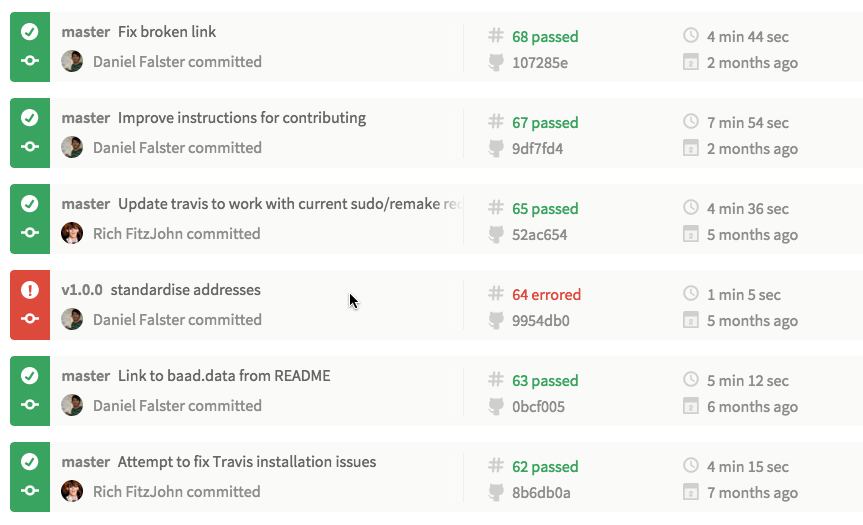
\includegraphics[width=\paperwidth]{shots/travis_builds}%
  }
  \bottomleft{\href{https://travis-ci.org/richfitz/wood/builds}{https://travis-ci.org/richfitz/wood/builds}}
\end{frame}

\begin{frame}
  \minionhigh{Find out what/who broke the project}
  \bottomhanging{%
    \includegraphics<1>[width=\paperwidth]{shots/travis_broken1}%
    \includegraphics<2>[width=\paperwidth]{shots/travis_broken2}}
\end{frame}

\begin{frame}
  \herohigh{\color{b-purple} Remake}
  \bottomhanging{

  }
\end{frame}

\begin{frame}
  \herohigh{\color{b-purple} Entirely open}
  \bottomhanging{
    \includegraphics<1>[width=.85\paperwidth]{pics/baad/F2015.png}
    \includegraphics<2>[width=.95\paperwidth]{snippets/baad_package}
  }
\end{frame}

\begin{frame}
  \herohigh{\color{b-purple} Started open}
  \bottomhanging{
    Would you like to publish
  }
\end{frame}

\begin{frame}
  \herohigh{\color{b-blue}Resources}
  \begin{tikzpicture}[remember picture, overlay]%
    \node[anchor=north west,align=left,font=\small] at
    ($(current page.west) + (0.05\paperwidth, .17\paperheight)$) {
      \begin{tabular}{>{\color{white}}r >{\color{b-grey}\footnotesize}l}
      Blog post &
      \hrefp{http}{ropensci.org/blog/2015/06/03/baad/}\\      
      Paper &
      \hrefp{http}{doi.org/10.1890/14-1889.1}\\
      Code &
      \hrefp{https}{github.com/dfalster/baad}\\
      Baad.data&
      \hrefp{https}{github.com/traitecoevo/baad.data}\\
      Remake &
      \hrefp{https}{github.com/richfitz/remake}\\
      Analysis & \hrefp{https}{github.com/RemkoDuursma/baadanalysis}\\
    \end{tabular}
  };
  \end{tikzpicture}
\end{frame}

\end{document}

%%% Local Variables:
%%% mode: latex
%%% TeX-PDF-mode: t
%%% TeX-engine: xetex
%%% End:
